\chapter{Resultados}

%\epsfig{file=imagenes/MaxMin0.eps, angle=-90, width=0.8\textwidth}
%\epsfig{file=fish01.ps, height=4cm, angle=-90} 

Con el simulador de ejecución de flujos de trabajo visto en el capítulo anterior, es necesario proponer un estudio con el objetivo de verificar la correcta funcionalidad del simulador y también con el objetivo de comparar los algoritmos de planificación implementados del simulador. A continuación, se discutirá sobre el diseño del experimento y se darán detalles sobre los resultados de la planificación de un flujo de trabajo en particular.

\section{Diseño del experimento}

Para probar los algoritmos, se hicieron varias pruebas con diferentes flujos de trabajo. En total, los tres algoritmos fueron ejecutados para planificar 50 flujos de trabajo generados aleatoriamente. Cada flujo de trabajo generado consta de 10 tareas y 12 dependencias entre tareas, las cuales se eligieron aleatoriamente y siempre verificando que cada dependencia no alterara la propiedad de que el flujo de trabajo sea un grafo dirigido acíclico. Los algoritmos fueron planificados en 3 recursos cuyos factores de velocidad se encuentran en la tabla \ref{table:resources}.

\begin{table}
\begin{center}
\begin{tabular}{|l|l|}
\hline
Nombre&Factor de velocidad\\
\hline
r1&7.373924\\
\hline
r2&2.540241\\
\hline
r3&4.530177\\
\hline
\end{tabular}
\end{center}
\label{table:resources}
\caption{Recursos utilizados para las pruebas de los algoritmos de planificación.}
\end{table}

En cada ejecución de cada algoritmo con cada flujo de trabajo se midió el tiempo total de ejecución, con el fin de comparar cada algoritmo y determinar cuál es el que genera las planificaciones con el menor tiempo total de ejecución. En la figura \ref{fig:tiempos_promedios} están graficados el tiempo total promedio de ejecución de cada algoritmo en los 50 flujos de trabajo aleatorios. Las barras de error en cada gráfica indican la desviación estándar del tiempo de ejecución por cada algoritmo.

\begin{figure}
\begin{center}
  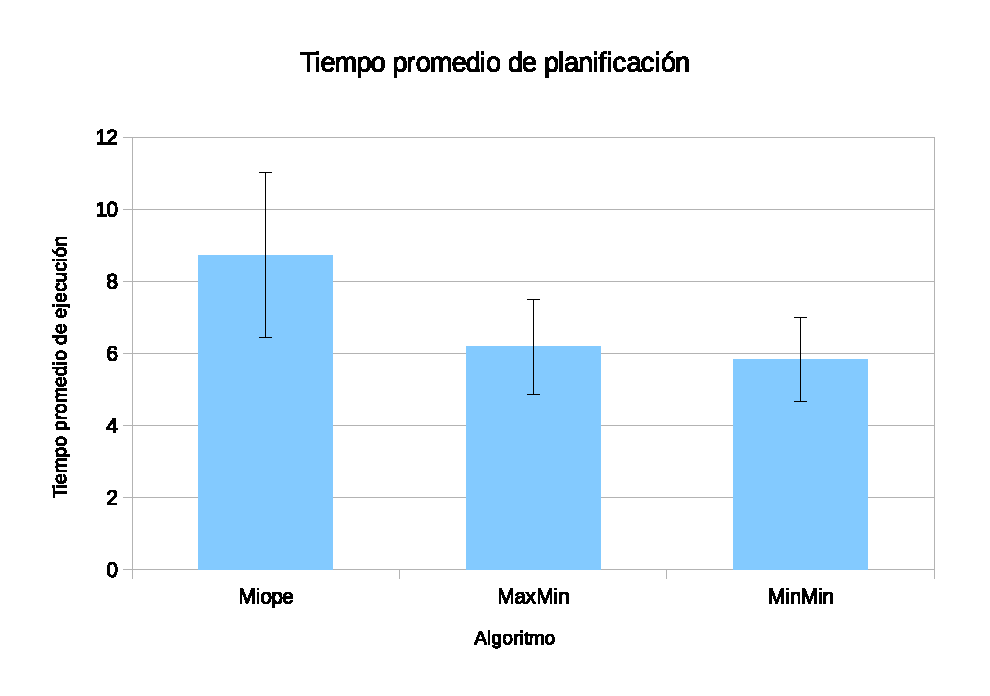
\epsfig{file=imagenes/tiempos_promedios.eps, width=0.8\textwidth}
\end{center}
\label{fig:tiempos_promedios}
\caption{Tiempos totales promedios de ejecución de cada algoritmo.}
\end{figure}

En la gráfica de la figura \ref{fig:tiempos_promedios} se puede apreciar que el algoritmo Miope tiene el mayor tiempo total promedio de ejecución. Luego, el algoritmo MaxMin y el algoritmo MinMin tienen los tiempos de ejecución menores que algoritmo Miope, siendo el algoritmo MinMin con el menor tiempo total promedio de planificación.

Sin embargo, las barras de error dan la idea de que hay una gran variabilidad en los resultados, lo cual podría indicar que existan algunos casos en los que el algoritmo Miope podría menores tiempos totales de planificación. Este hecho es aún más notorio para los algoritmos MaxMin y MinMin. Esto es más notorio en la gráfica de la figura \ref{fig:tiempos_totales}, donde se puede ver, por ejemplo, que en el flujo de trabajo núm. 20, el algoritmo Miope tiene un menor tiempo de planificación que el algoritmo MaxMin.

\begin{figure}
\begin{center}
  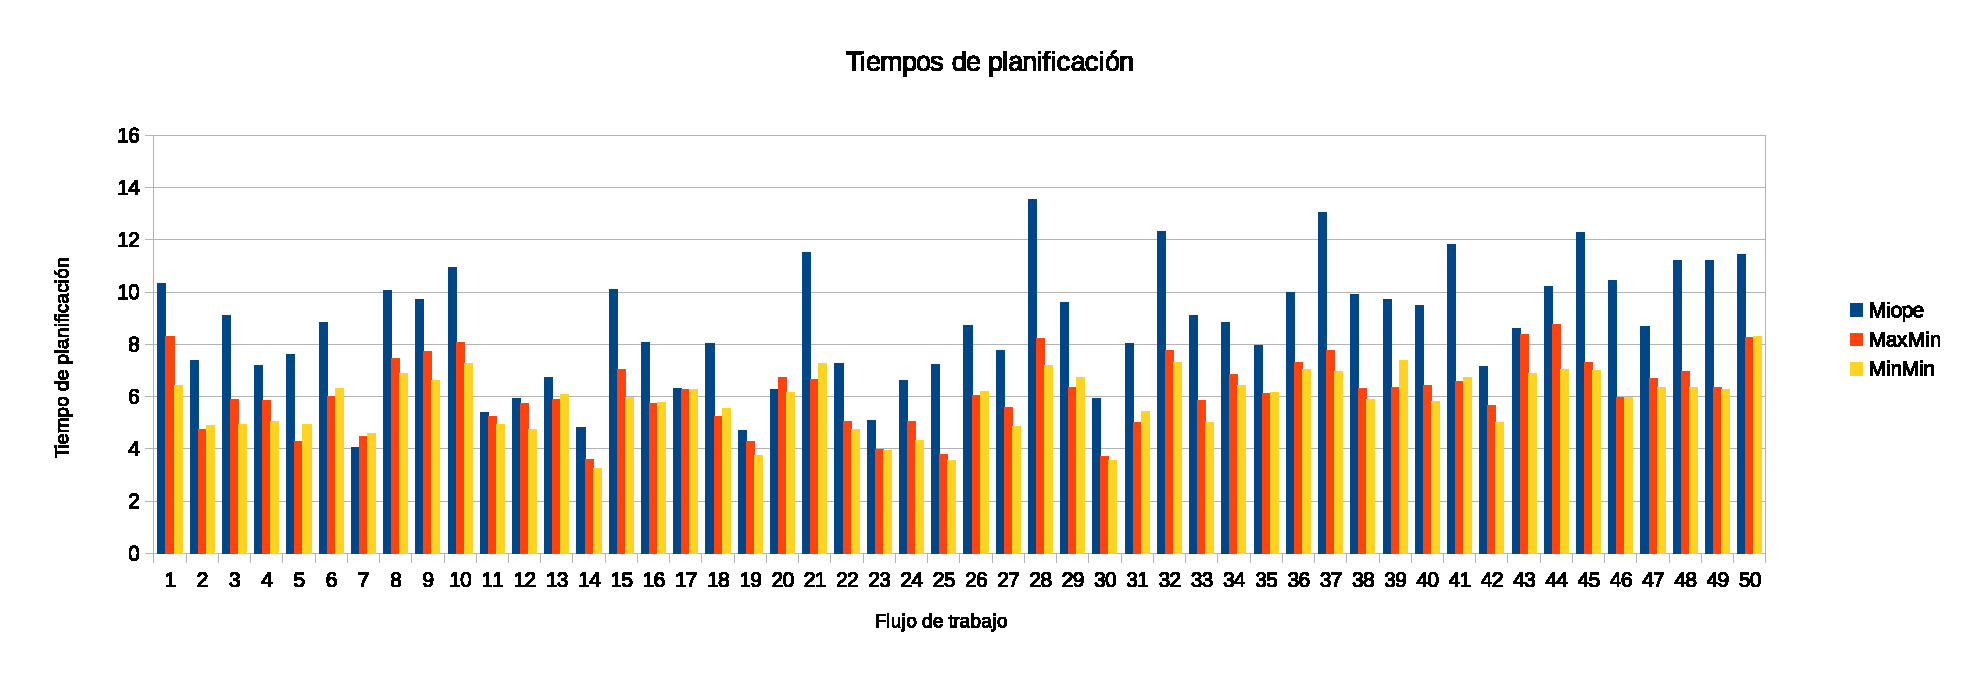
\epsfig{file=imagenes/tiempos_totales.eps, height=6cm, angle=90}
\end{center}
\label{fig:tiempos_totales}
\caption{Tiempos totales de ejecución de cada algoritmo en cada flujo de trabajo aleatorio.}
\end{figure}

\section{Análsis del flujo de trabajo número 7}
Para saber por qué ocurre el fenómeno descrito en el párrafo anterior, se estudiarán a detalle las planificaciones que produce cada algoritmo y la estructura del flujo de trabajo número 7. En la figura \ref{fig:workflow6} se puede ver este flujo de trabajo. Los nodos cuyo color es azul fuerte tienen un factor de complejidad más alto que los nodos con color azul claro.

\begin{figure}
\begin{center}
  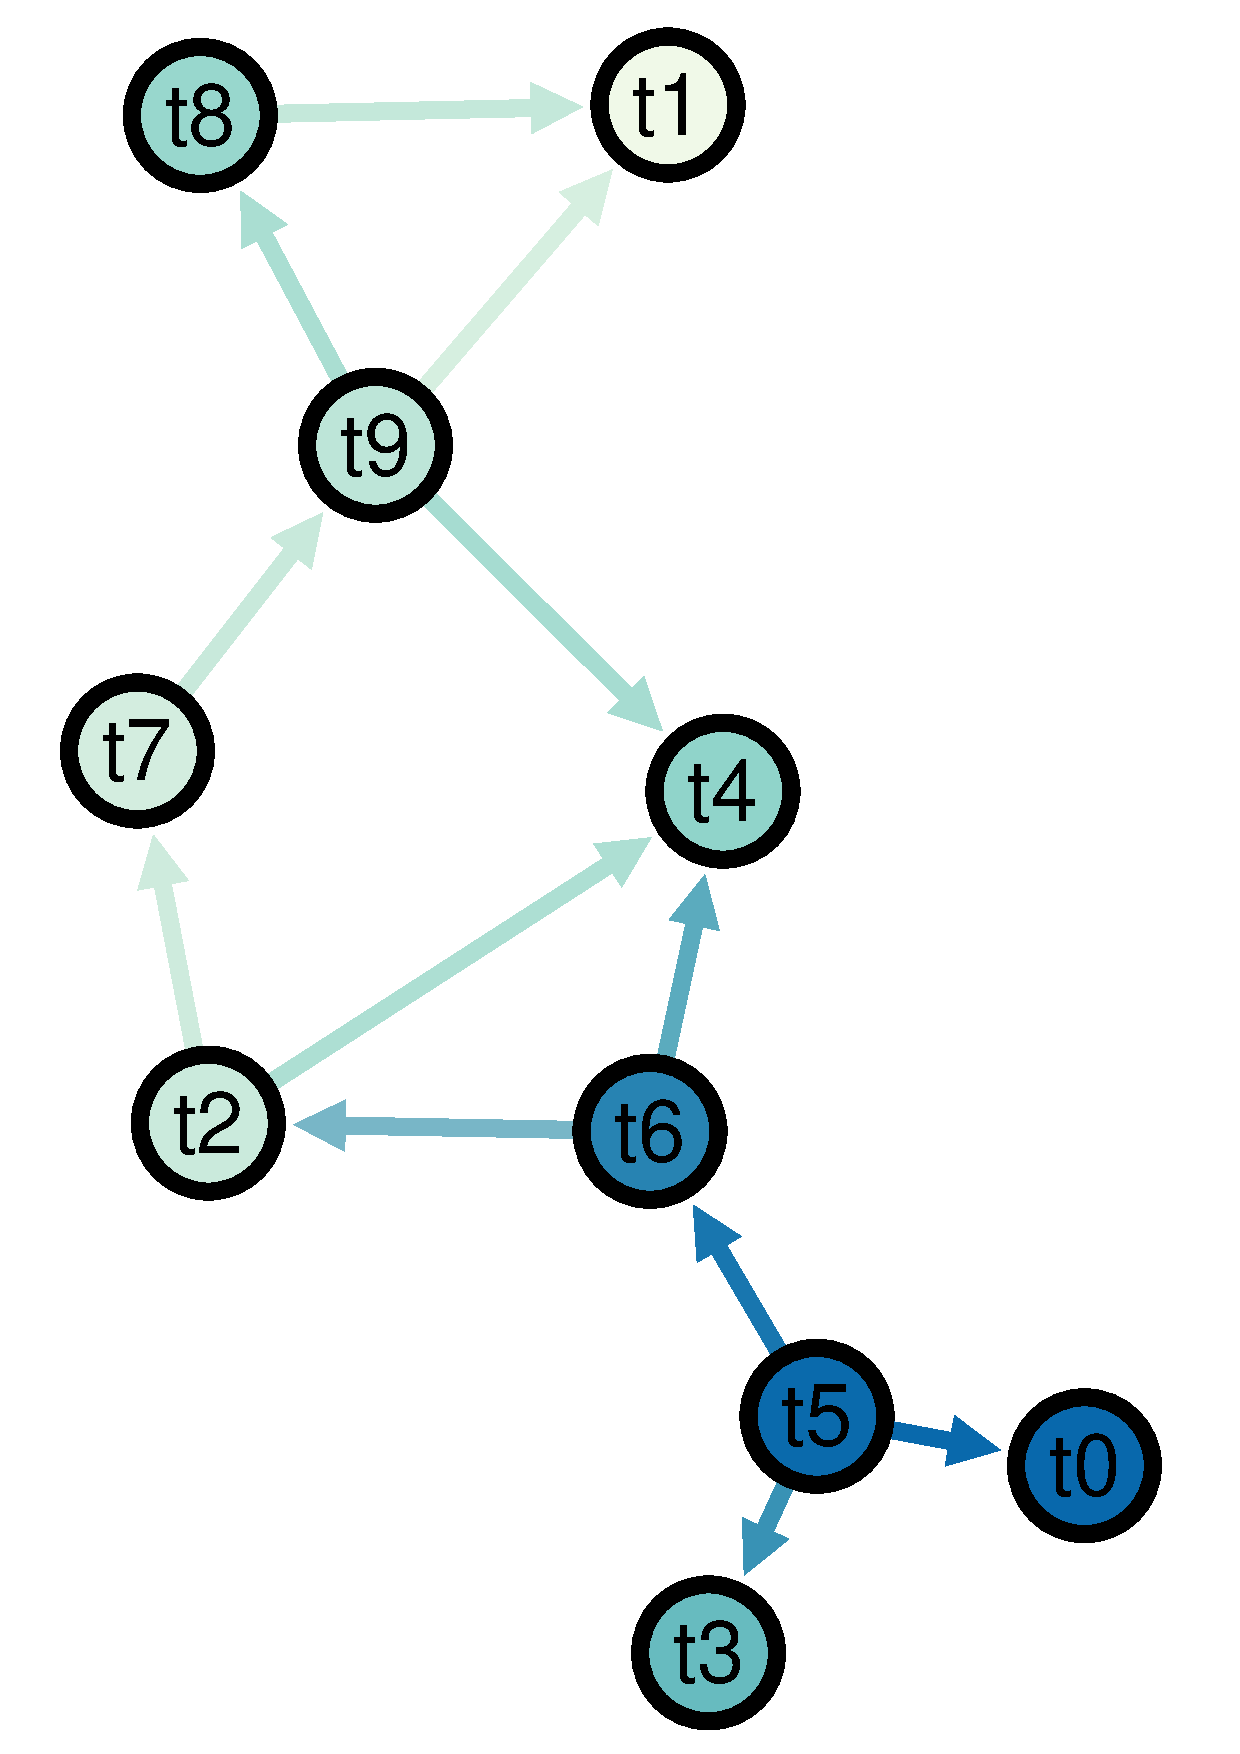
\includegraphics[width=0.5\textwidth]{imagenes/workflow6.pdf}
\end{center}
\label{fig:workflow6}
\caption{Flujo de trabajo número 7, generado aleatoriamente}
\end{figure}

Ahora, en la figura \ref{fig:schedules6} están representadas las planificaciones que dan como salida los algoritmos Miope, MaxMin y MinMin, respectivamente. En el eje vertical están los recursos que se ocupan en el flujo de trabjo. En el eje horizontal indica el tiempo y los cuadros de color representan la duración de las tareas en cada recurso. Cabe aclarar que los tiempos totales de ejecución de las planificaciones de los algoritmos Miope, MaxMin y MinMin fueron 4.063928  4.471435 y 4.569478, respectivamente.

\begin{figure}
\begin{center}
  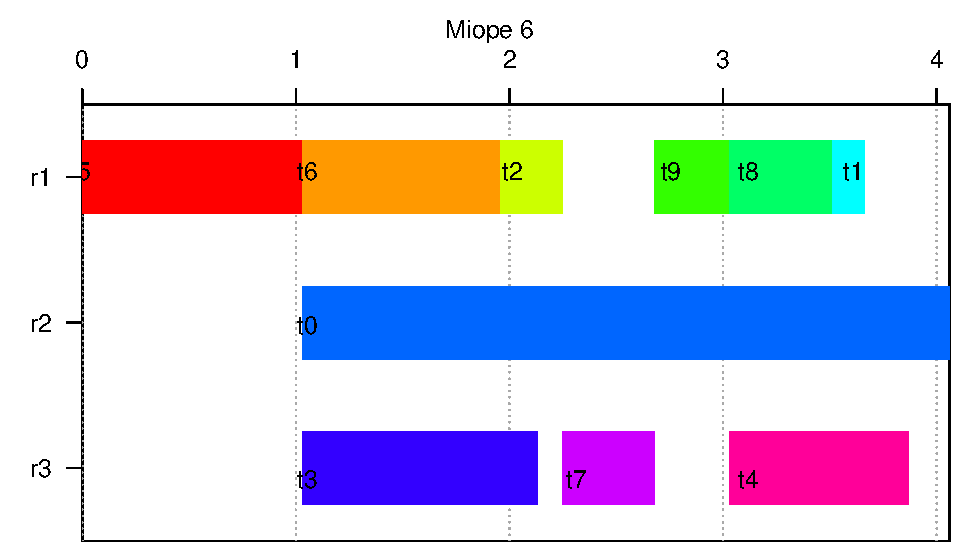
\includegraphics[width=0.3\textwidth]{imagenes/Myopic6.pdf}
  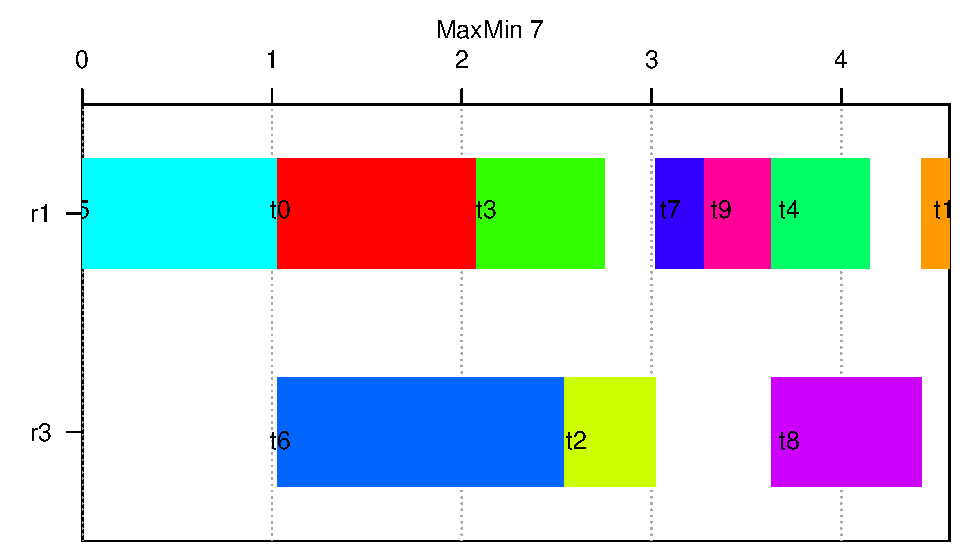
\includegraphics[width=0.3\textwidth]{imagenes/MaxMin6.pdf}
  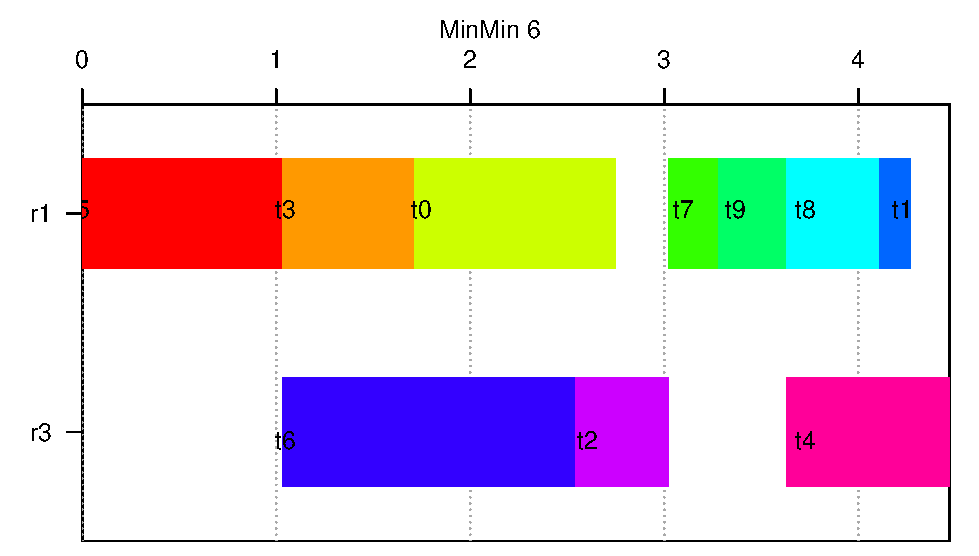
\includegraphics[width=0.3\textwidth]{imagenes/MinMin6.pdf}
\end{center}
\label{fig:schedules6}
\caption{Planificaciones de cada uno de los algoritmos para el flujo de trabajo número 7.}
\end{figure}

En las planificaciones, se puede ver que el algoritmo Miope asignó la tarea $t0$ al recurso $r2$, que es el recurso más lento. Por otro lado, los algoritmos MaxMin y MinMin no utilizaron el recurso $r2$. Esto se debe a que ambos algoritmos buscan minimizar el tiempo de ejecución de cada tarea en cada recurso. Como el recurso $r2$ es el que tiene el menor factor de velocidad, el $ECT(t,r)$ que calculan los algoritmos MaxMin y MinMin es muy alto, por lo que nunca se elige el recurso $r2$. Finalmente, en los demás casos, se puede ver la tendencia de que MinMin obtiene los tiempos totales de planificación más pequeños, seguido de MaxMin y luego del algoritmo Miope. 

Para verificar este resultado, se realizaron tres pruebas T de hipótesis de cola superior con una muestra de tamaño $n=50$. Estas pruebas se hicieron sobre las diferencias de los tiempos totales de ejecución entre los algoritmos. Así, sean $D_1 = T_{Miope} - T_{MaxMin}$, $D_2 = T_{Miope} - T_{MinMin}$, $D_3 = T_{MaxMin} - T_{MinMin}$ las diferencias entre tiempos totales de ejecución. La hipótesis nula para cada prueba es $H_0: \overline{T_i} = 0, i=\{1,2,3\}$, y la hipótesis alternativa es $H_a: \overline{T_i} > 0, i=\{1,2,3\}$. De este modo, los valores-p para cada prueba de hipótesis son: $4.040898 \times 10^{-16}$ $3.573361 \times 10^{-18}$ y $6.750317 \times 10^{-5}$. Estos valores p son muy pequeños, por lo que se puede rechazar la hipótesis nula hasta con un nivel de confianza del 99\%. Por lo tanto, hay una diferencia positiva entre los tiempos de ejecución de cada algoritmo, siendo el algoritmo MinMin el que obtiene, en promedio, los tiempos totales de ejecución más cortos.

